\documentclass{article}
\usepackage{iclr2025_conference,times}
\input{math_commands.tex}

\usepackage{hyperref}
\usepackage{url}
\usepackage{graphicx}
\usepackage{booktabs}
\usepackage{amsmath}
\usepackage{float}
\usepackage{subcaption}

%\iclrfinalcopy % removed: we want line numbers (submission mode) with visible authors

\title{Explainable AI Analysis on Cross-View Geo-Localization\\with Sample4Geo}

\author{
Kuzey Ersoy (2230356168)\thanks{Equal contribution.} \quad \.{I}sa Halis Y\"{u}cel (2220356137)\footnotemark[1] \\
Department of Computer Engineering\\
Hacettepe University\\
Ankara, T\"{u}rkiye\\
\texttt{\{b2230356168, b2220356137\}@cs.hacettepe.edu.tr}
}

\begin{document}

\maketitle

\vspace{-0.5em}
\noindent\textbf{Video:} \url{https://www.youtube.com/watch?v=PLACEHOLDER}\\
\textbf{Code \& Weights:} \url{https://github.com/halisyucel/Sample4Geo}\\
\textbf{Datasets:} \url{https://drive.google.com/drive/folders/1m85pmQhE_iMRUbc173Z81Gs3ID5-wD2C?usp=sharing}

\begin{abstract}
Cross-view geo-localization matches query images from ground-level or aerial platforms against georeferenced satellite databases.
While state-of-the-art methods such as Sample4Geo achieve strong retrieval accuracy, their decision processes remain opaque.
This work applies two complementary Explainable AI (XAI) methods, namely Grad-CAM (gradient-based, white-box) and Occlusion Sensitivity (perturbation-based, black-box), to a pretrained Sample4Geo model across two benchmarks: University-1652 (drone-to-satellite) and VIGOR (street-to-satellite).
We analyze eight distinct scenarios (two datasets $\times$ two methods $\times$ successful/failed matches) and quantify explanation quality via faithfulness curves.
Our analysis reveals that successful matches anchor on cross-view invariant structures (building footprints, road junctions), while failures exhibit diffuse attention or fixation on view-dependent features invisible from the opposite perspective.
\end{abstract}

%──────────────────────────────────────────────────────────────────────────────
\section{Introduction}
\label{sec:intro}

Cross-view geo-localization determines the geographic location of a query image by matching it against a georeferenced satellite database.
This is essential for autonomous navigation in GPS-denied environments.
The task is challenging because query and gallery images are captured from drastically different viewpoints (drone or street-level versus overhead satellite), introducing severe geometric and appearance discrepancies.

Deep metric learning approaches, particularly Sample4Geo~\citep{deuser2023sample4geo}, achieve state-of-the-art retrieval accuracy by learning view-invariant embeddings via contrastive losses.
However, these models operate as black boxes: high retrieval scores do not reveal \emph{which} image regions drive the matching decision.
Understanding spatial reasoning is critical for diagnosing failure modes, building trust, and guiding architectural improvements.

We apply two fundamentally different XAI methods to a pretrained Sample4Geo model across two complementary datasets.
Our contributions: (1) systematic XAI evaluation across 8 scenarios with qualitative heatmaps and quantitative faithfulness metrics; (2) identification of two failure modes, \emph{diffuse gallery attention} and \emph{cross-view invisible features}; (3) demonstration that both XAI methods converge on the same regions, providing mutual validation.

%──────────────────────────────────────────────────────────────────────────────
\section{Methods}
\label{sec:methods}

\subsection{Sample4Geo Architecture}

Sample4Geo~\citep{deuser2023sample4geo} employs a weight-sharing Siamese architecture with a ConvNeXt-Base~\citep{liu2022convnext} backbone pretrained on ImageNet-22k~\citep{deng2009imagenet}.
Both query and gallery images are projected into a shared 1024-dimensional embedding space via a Symmetric InfoNCE loss~\citep{oord2018infonce}:
\begin{equation}
    \mathcal{L}_{\text{InfoNCE}} = -\log \frac{\exp\bigl(\text{sim}(q, k^+)/\tau\bigr)}{\sum_{i=0}^{K} \exp\bigl(\text{sim}(q, k_i)/\tau\bigr)}
    \label{eq:infonce}
\end{equation}
where $\text{sim}(q, k)$ is cosine similarity, $k^+$ is the positive match, and $\tau$ is a temperature parameter.
At inference, retrieval ranks gallery images by cosine similarity to the query embedding.

\subsection{Grad-CAM}

Grad-CAM~\citep{selvaraju2017gradcam} produces a spatial heatmap by backpropagating the cosine similarity score through the network.
Importance weights $\alpha_k$ are computed by global average pooling the gradients into the last convolutional stage:
\begin{equation}
    L_{\text{Grad-CAM}} = \text{ReLU}\left(\sum_k \alpha_k A^k\right), \quad \alpha_k = \frac{1}{Z}\sum_i\sum_j \frac{\partial \text{sim}(q,g)}{\partial A^k_{ij}}
    \label{eq:gradcam}
\end{equation}
We target the last block of ConvNeXt Stage~4, producing $12\times12$ maps upsampled to $384\times384$.

\subsection{Occlusion Sensitivity}

Occlusion Sensitivity~\citep{zeiler2014visualizing} systematically slides a gray patch ($P{\times}P$ pixels, stride $S$) across the input and records the cosine similarity drop at each position:
\begin{equation}
    I(y, x) = \text{sim}_{\text{base}} - \text{sim}_{\text{occluded}(y,x)}
    \label{eq:occlusion}
\end{equation}
We use $P{=}64$, $S{=}32$ on $384{\times}384$ inputs, yielding $11^2{=}121$ positions per image, batched in groups of 32 for efficiency (4 forward passes per image).

\subsection{Faithfulness Evaluation}

We compute faithfulness curves~\citep{petsiuk2018rise} by ranking pixels by importance, progressively masking the top-$k\%$ (10 steps), and measuring the resulting cosine similarity.
A faithful explanation yields a monotonically decreasing curve; non-monotonic behaviour indicates misleading feature attention.

%──────────────────────────────────────────────────────────────────────────────
\section{Experimental Settings}
\label{sec:settings}

\paragraph{University-1652}~\citep{zheng2020university} contains images of 1,652 university buildings from drone, satellite, and street-view perspectives.
We evaluate Drone-to-Satellite (D2S): 37,855 drone queries matched against 951 satellite gallery images.

\paragraph{VIGOR}~\citep{zhu2021vigor} pairs 360$^\circ$ street panoramas with satellite tiles across four US cities.
Same-area split: 52,605 queries / 90,618 gallery; Cross-area split: 53,694 queries / 46,563 gallery.
The extreme viewpoint gap (ground $\leftrightarrow$ overhead) makes this significantly harder.

\paragraph{Metrics.} Recall@$k$ ($k{\in}\{1,5,10\}$), Average Precision (U1652), and Hit Rate (VIGOR).

\paragraph{Implementation.} ConvNeXt-Base, $384{\times}384$ input, ImageNet normalization.
Pretrained weights from~\citet{deuser2023sample4geo}.
Feature extraction: batch size 256, 16 workers, NVIDIA A100-SXM4-40GB.
VIGOR similarity matrix computed via streaming chunks (size 1000) to fit GPU memory.
For XAI: 5 successful + 3 failed pairs per dataset.

%──────────────────────────────────────────────────────────────────────────────
\section{Experimental Results}
\label{sec:results}

\subsection{Baseline Verification}

Table~\ref{tab:baseline} reports retrieval performance.
U1652 R@1 (92.66\%) is ${\sim}2.5\%$ below the published 95.15\%, consistent across hardware, likely due to evaluation protocol differences.
VIGOR results match published values (77.86\% same-area, 61.71\% vs.\ 61.09\% cross-area).

\begin{table}[h]
\vspace{-0.5em}
\caption{Baseline retrieval performance of the pretrained Sample4Geo model.}
\label{tab:baseline}
\centering
\small
\begin{tabular}{lcccc}
\toprule
\textbf{Dataset / Split} & \textbf{R@1} & \textbf{R@5} & \textbf{R@10} & \textbf{AP / Hit Rate} \\
\midrule
University-1652 (D2S) & 92.66\% & 97.69\% & 98.24\% & 93.81\% (AP) \\
VIGOR Same-Area & 77.86\% & 95.68\% & 97.22\% & 89.83\% (HR) \\
VIGOR Cross-Area & 61.71\% & 83.51\% & 87.99\% & 69.87\% (HR) \\
\bottomrule
\end{tabular}
\vspace{-0.5em}
\end{table}

\subsection{Grad-CAM Analysis}

\paragraph{University-1652, Successful Matches (Figure~\ref{fig:gradcam_u1652}).}
The drone query focuses on \textbf{building edges and rooftop transitions}; the satellite gallery highlights the corresponding footprint.
All 5 pairs are from the same building (ID~0003, different drone angles), demonstrating viewpoint robustness.
Faithfulness curves decrease monotonically (${\sim}0.89 \to {\sim}0.32$), confirming correct feature identification.

\paragraph{University-1652, Failed Matches (Figure~\ref{fig:gradcam_u1652}).}
The query still localizes meaningful structures, but the wrong gallery image shows \textbf{diffuse, scattered activation} with no dominant anchor.
Gallery faithfulness is flat, confirming absent spatial correspondence.

\paragraph{VIGOR, Successful Matches (Figure~\ref{fig:gradcam_vigor}).}
Street queries focus on landmarks (facades, fences); the satellite gallery attends to corresponding road junctions.
Faithfulness shows downward trends with occasional non-monotonic bumps characteristic of the harder cross-view task.

\paragraph{VIGOR, Failed Matches (Figure~\ref{fig:gradcam_vigor}).}
A street view \textbf{under an elevated metro structure} causes the model to attend to overhead steel, which is invisible from satellite.
Faithfulness curves are V-shaped: masking \emph{improves} similarity, proving the features actively mislead.

\begin{figure}[t]
\centering
\begin{subfigure}[t]{0.49\linewidth}
    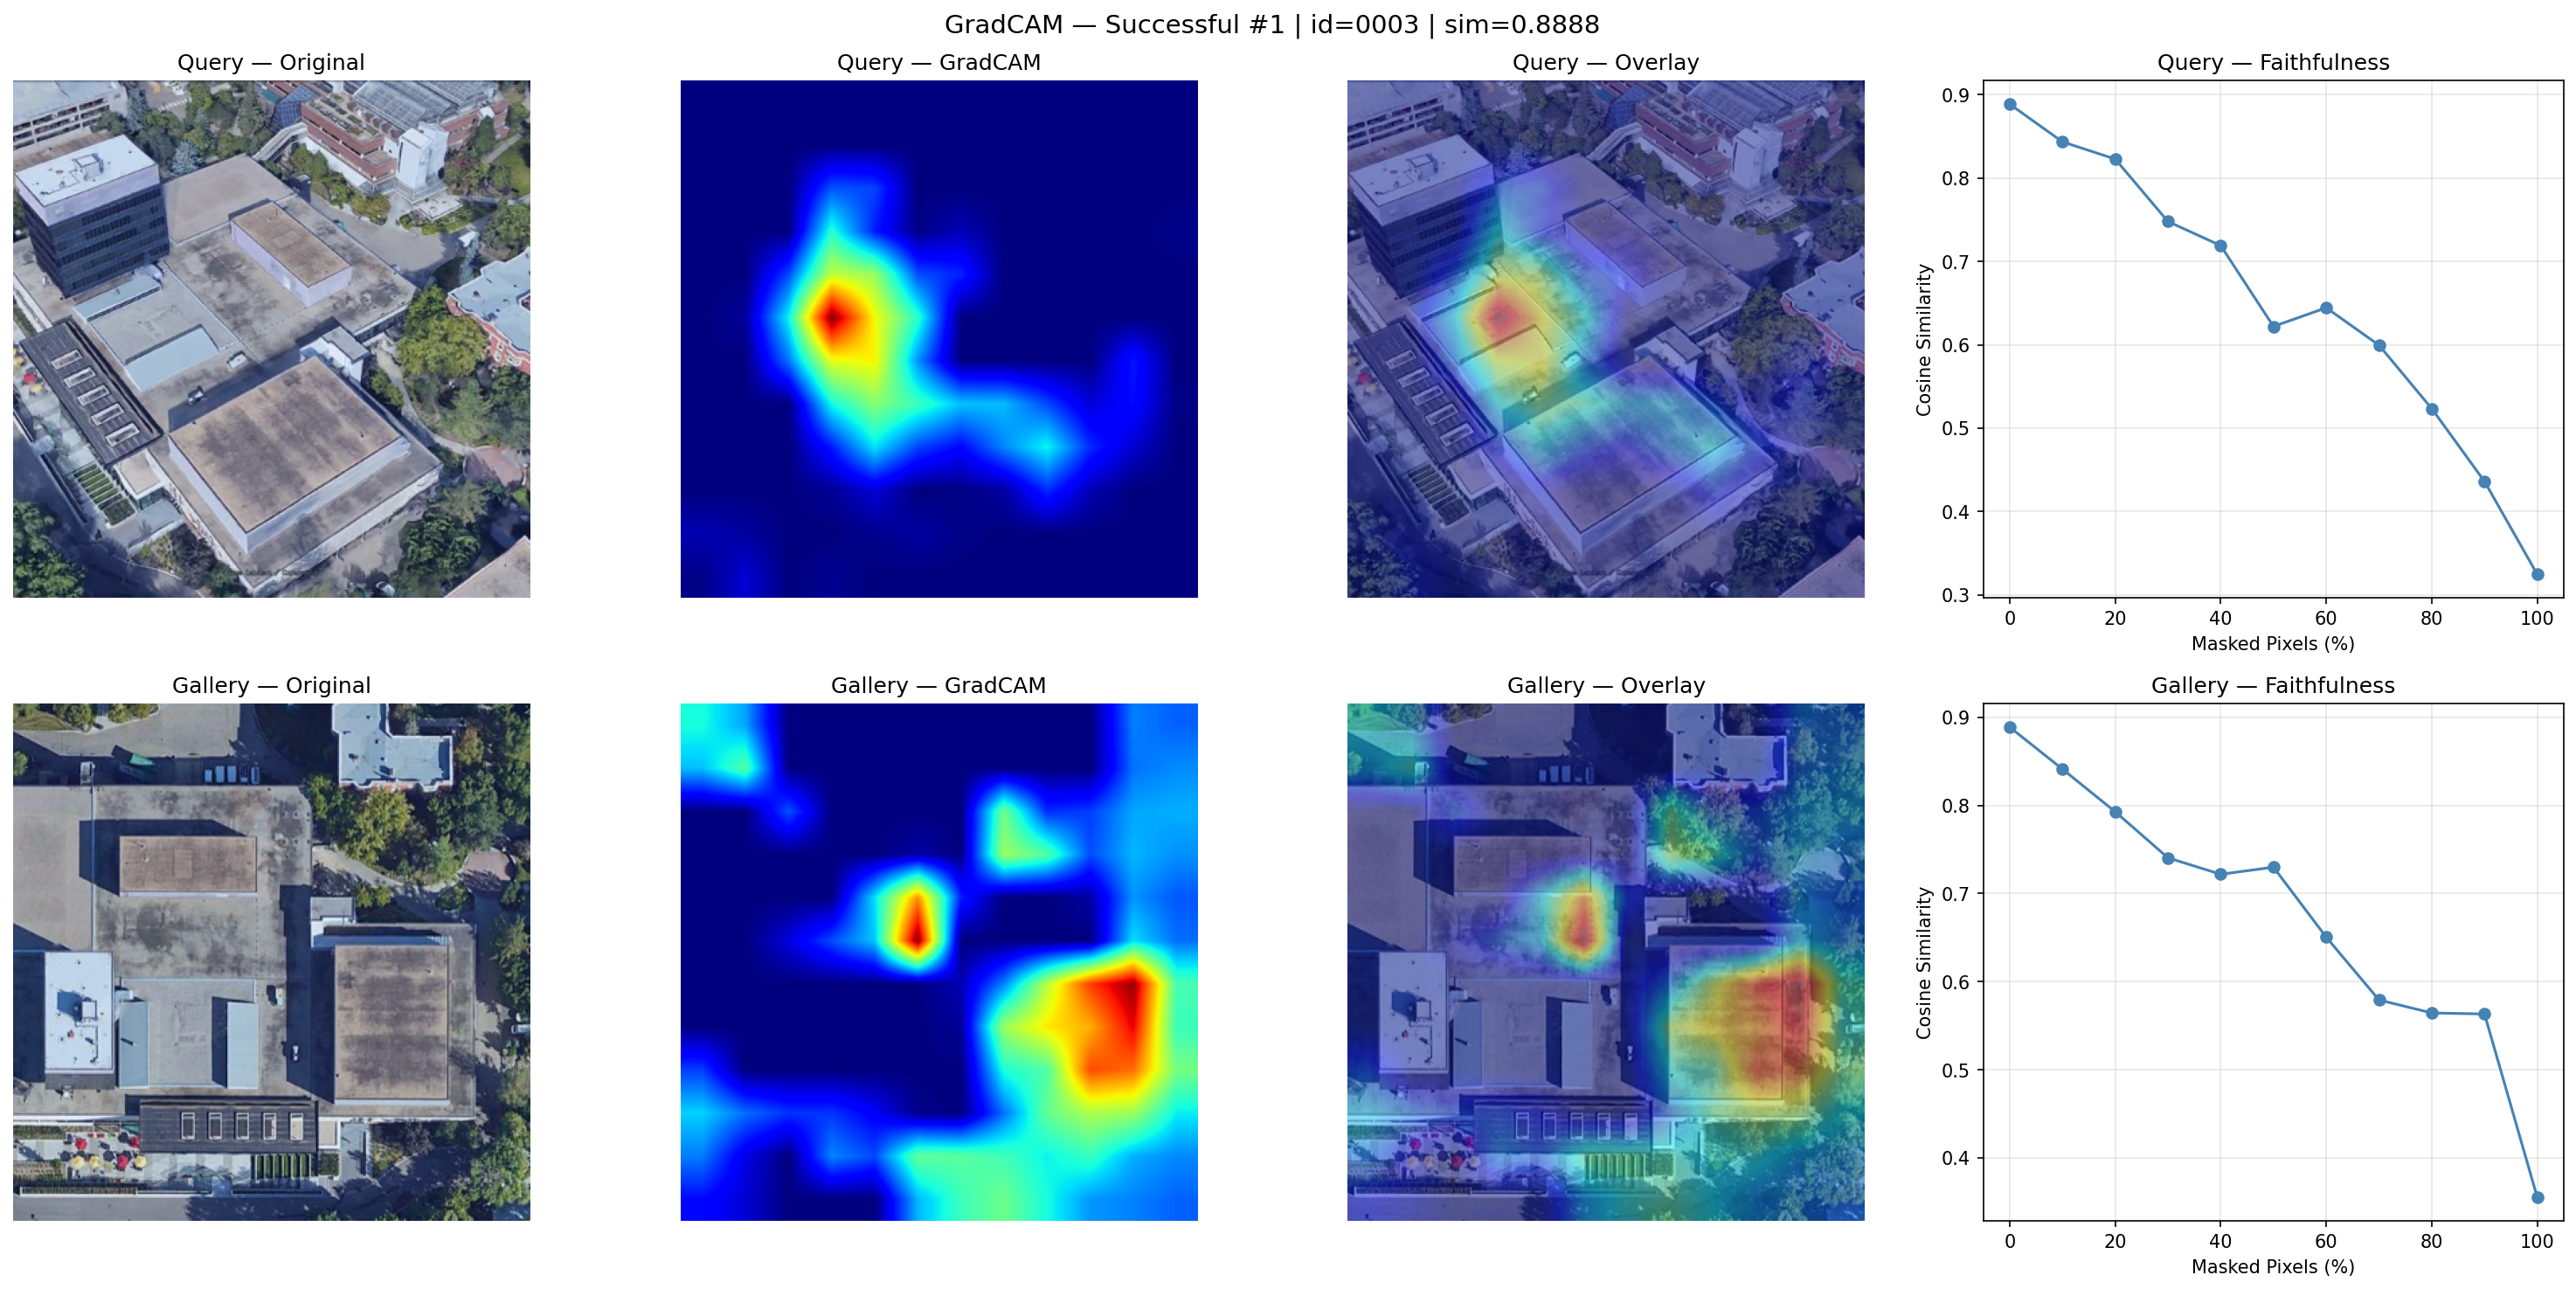
\includegraphics[width=\linewidth]{figures/gradcam/u1652_successful_01.png}
    \caption{Successful (ID=0003, sim=0.89)}
\end{subfigure}
\hfill
\begin{subfigure}[t]{0.49\linewidth}
    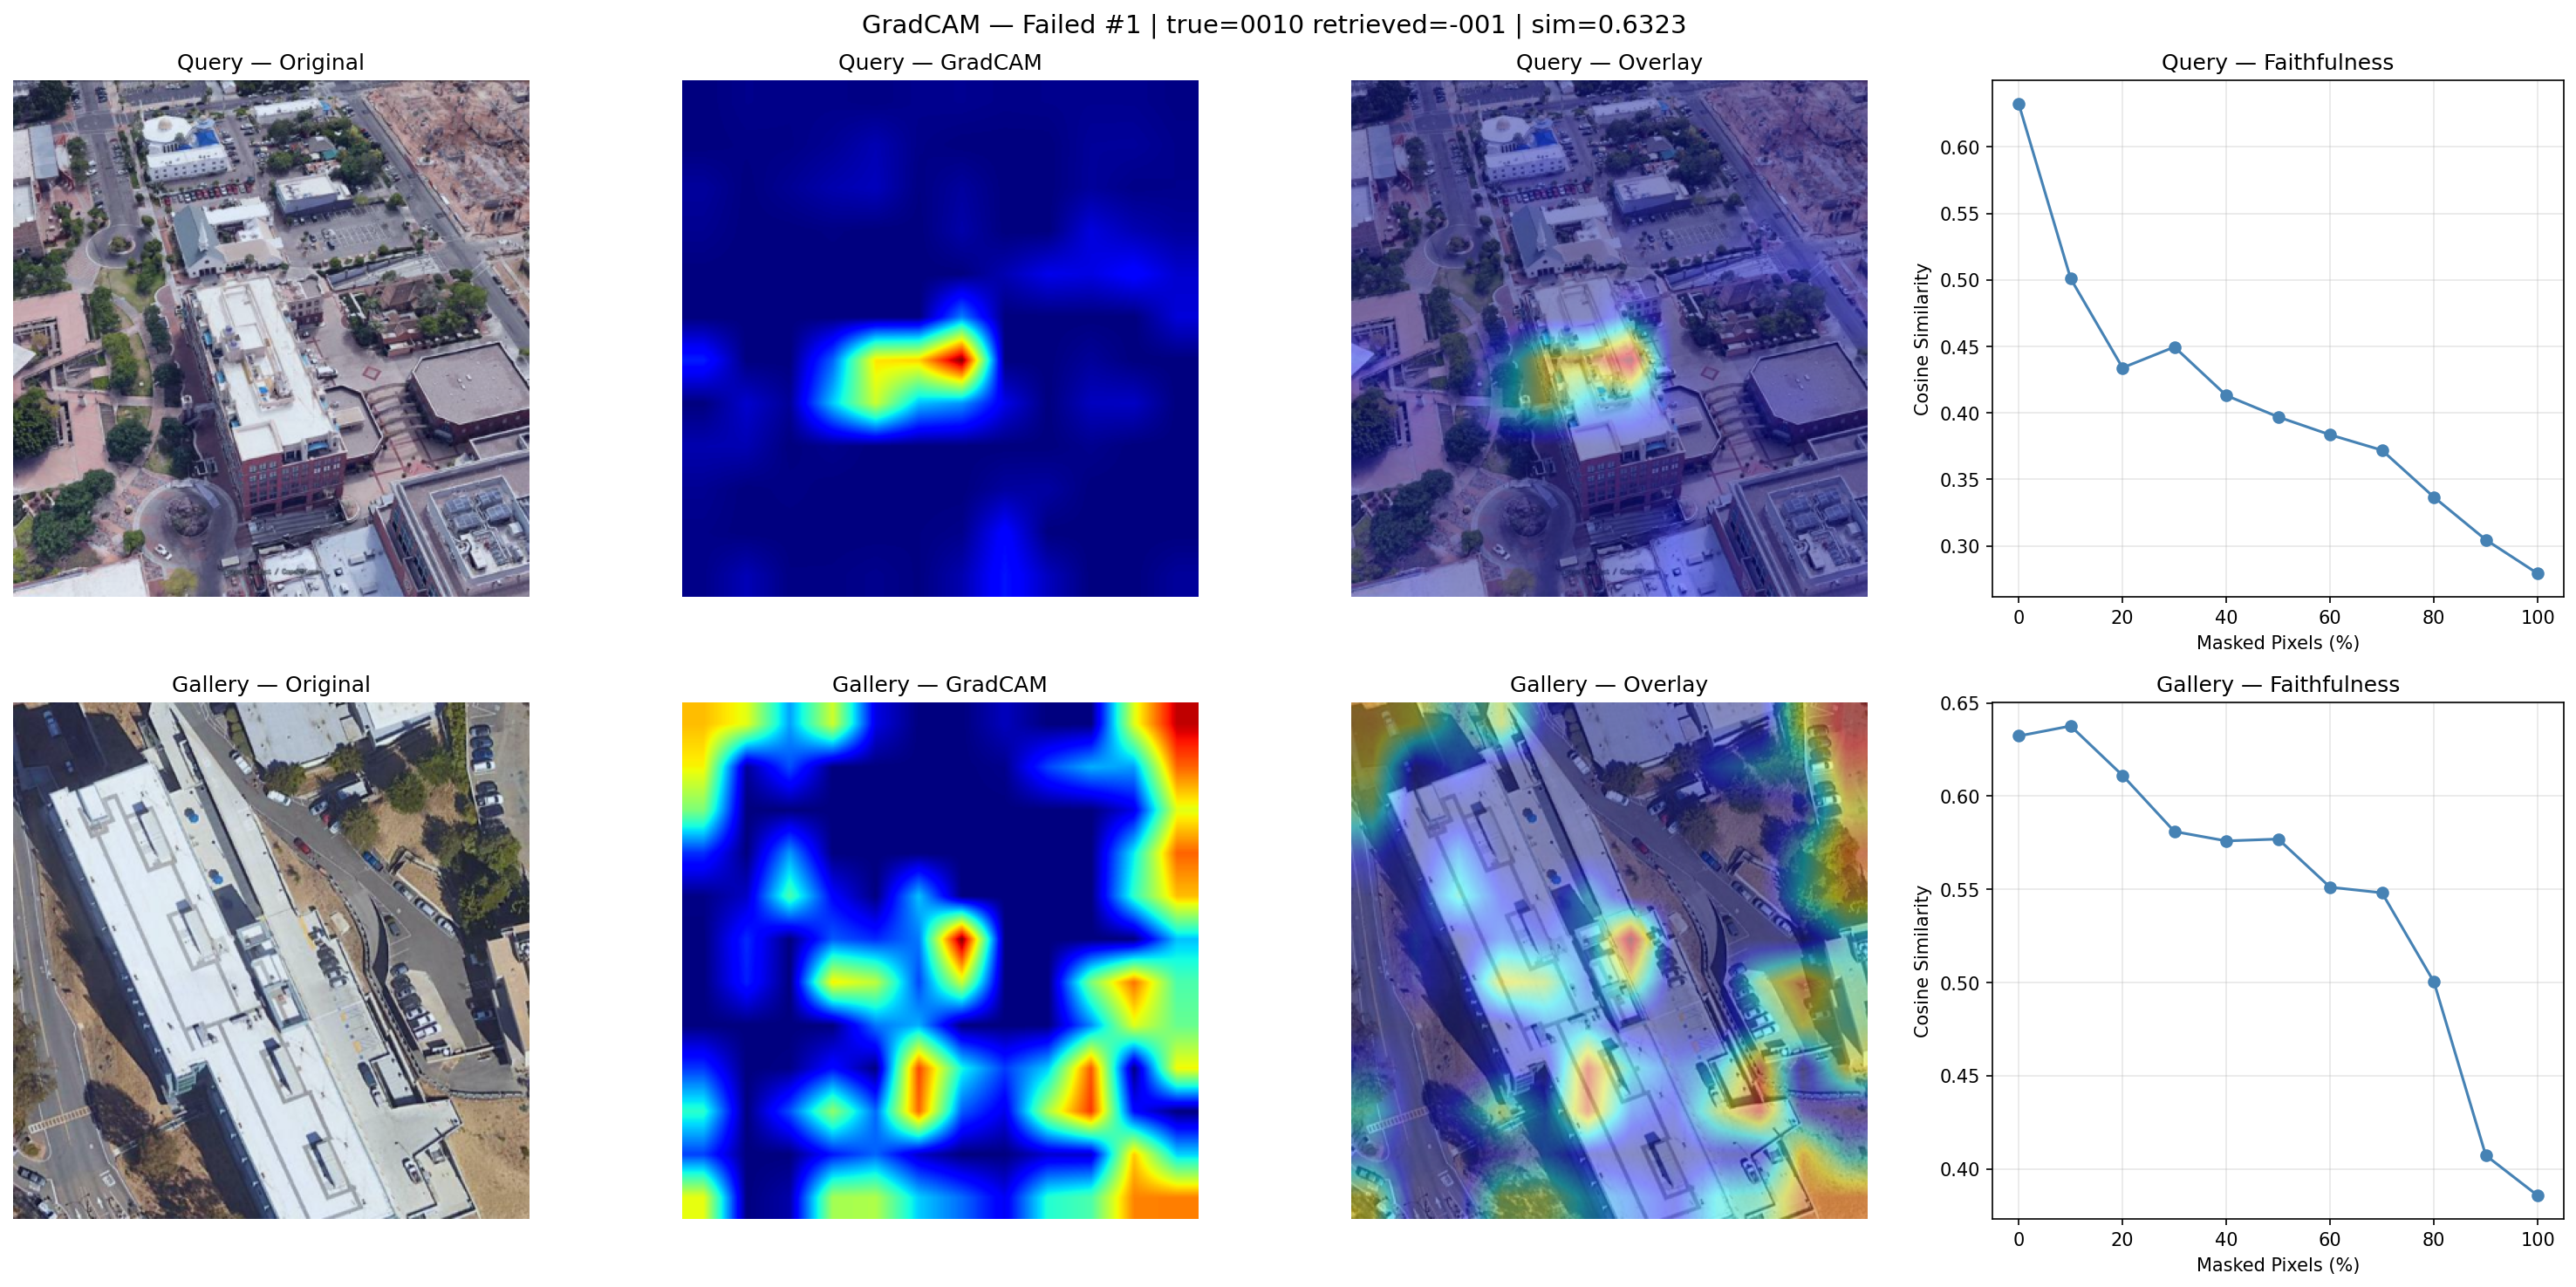
\includegraphics[width=\linewidth]{figures/gradcam/u1652_failed_01.png}
    \caption{Failed (true=0010, ret.=-001)}
\end{subfigure}
\caption{Grad-CAM on University-1652. (a) Successful: focused rooftop attention with monotonic faithfulness. (b) Failed: query has clear focus but gallery shows diffuse scattered activation.}
\label{fig:gradcam_u1652}
\end{figure}

\begin{figure}[t]
\centering
\begin{subfigure}[t]{0.49\linewidth}
    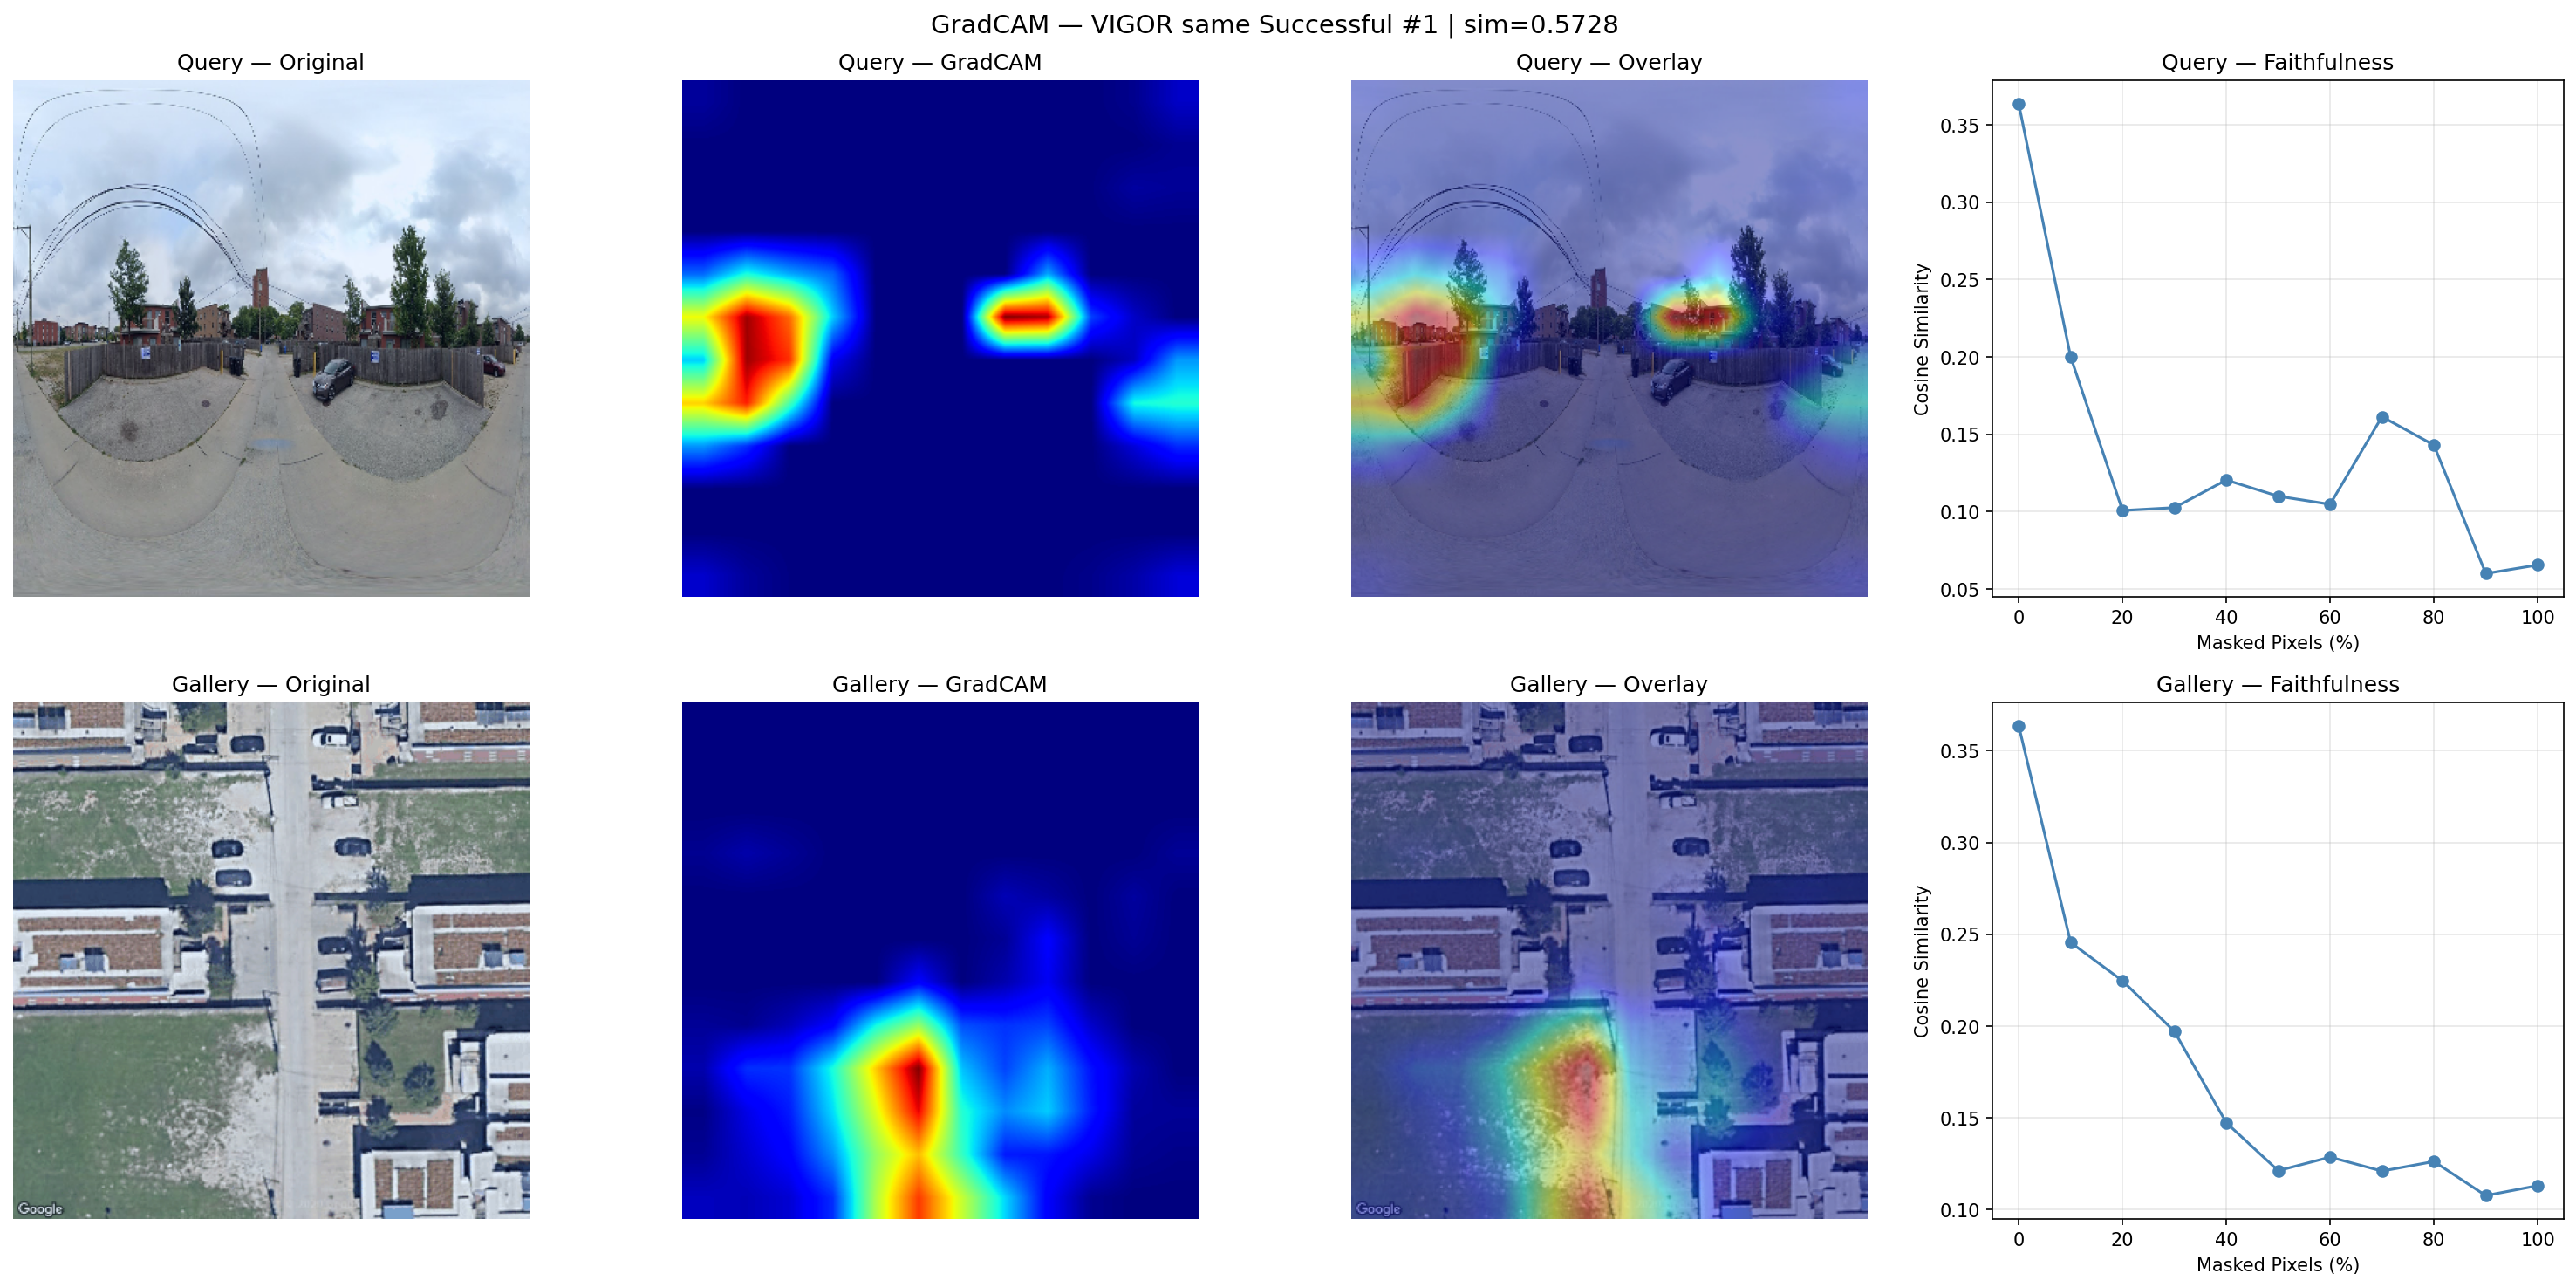
\includegraphics[width=\linewidth]{figures/gradcam/vigor_same_successful_01.png}
    \caption{Successful (sim=0.57)}
\end{subfigure}
\hfill
\begin{subfigure}[t]{0.49\linewidth}
    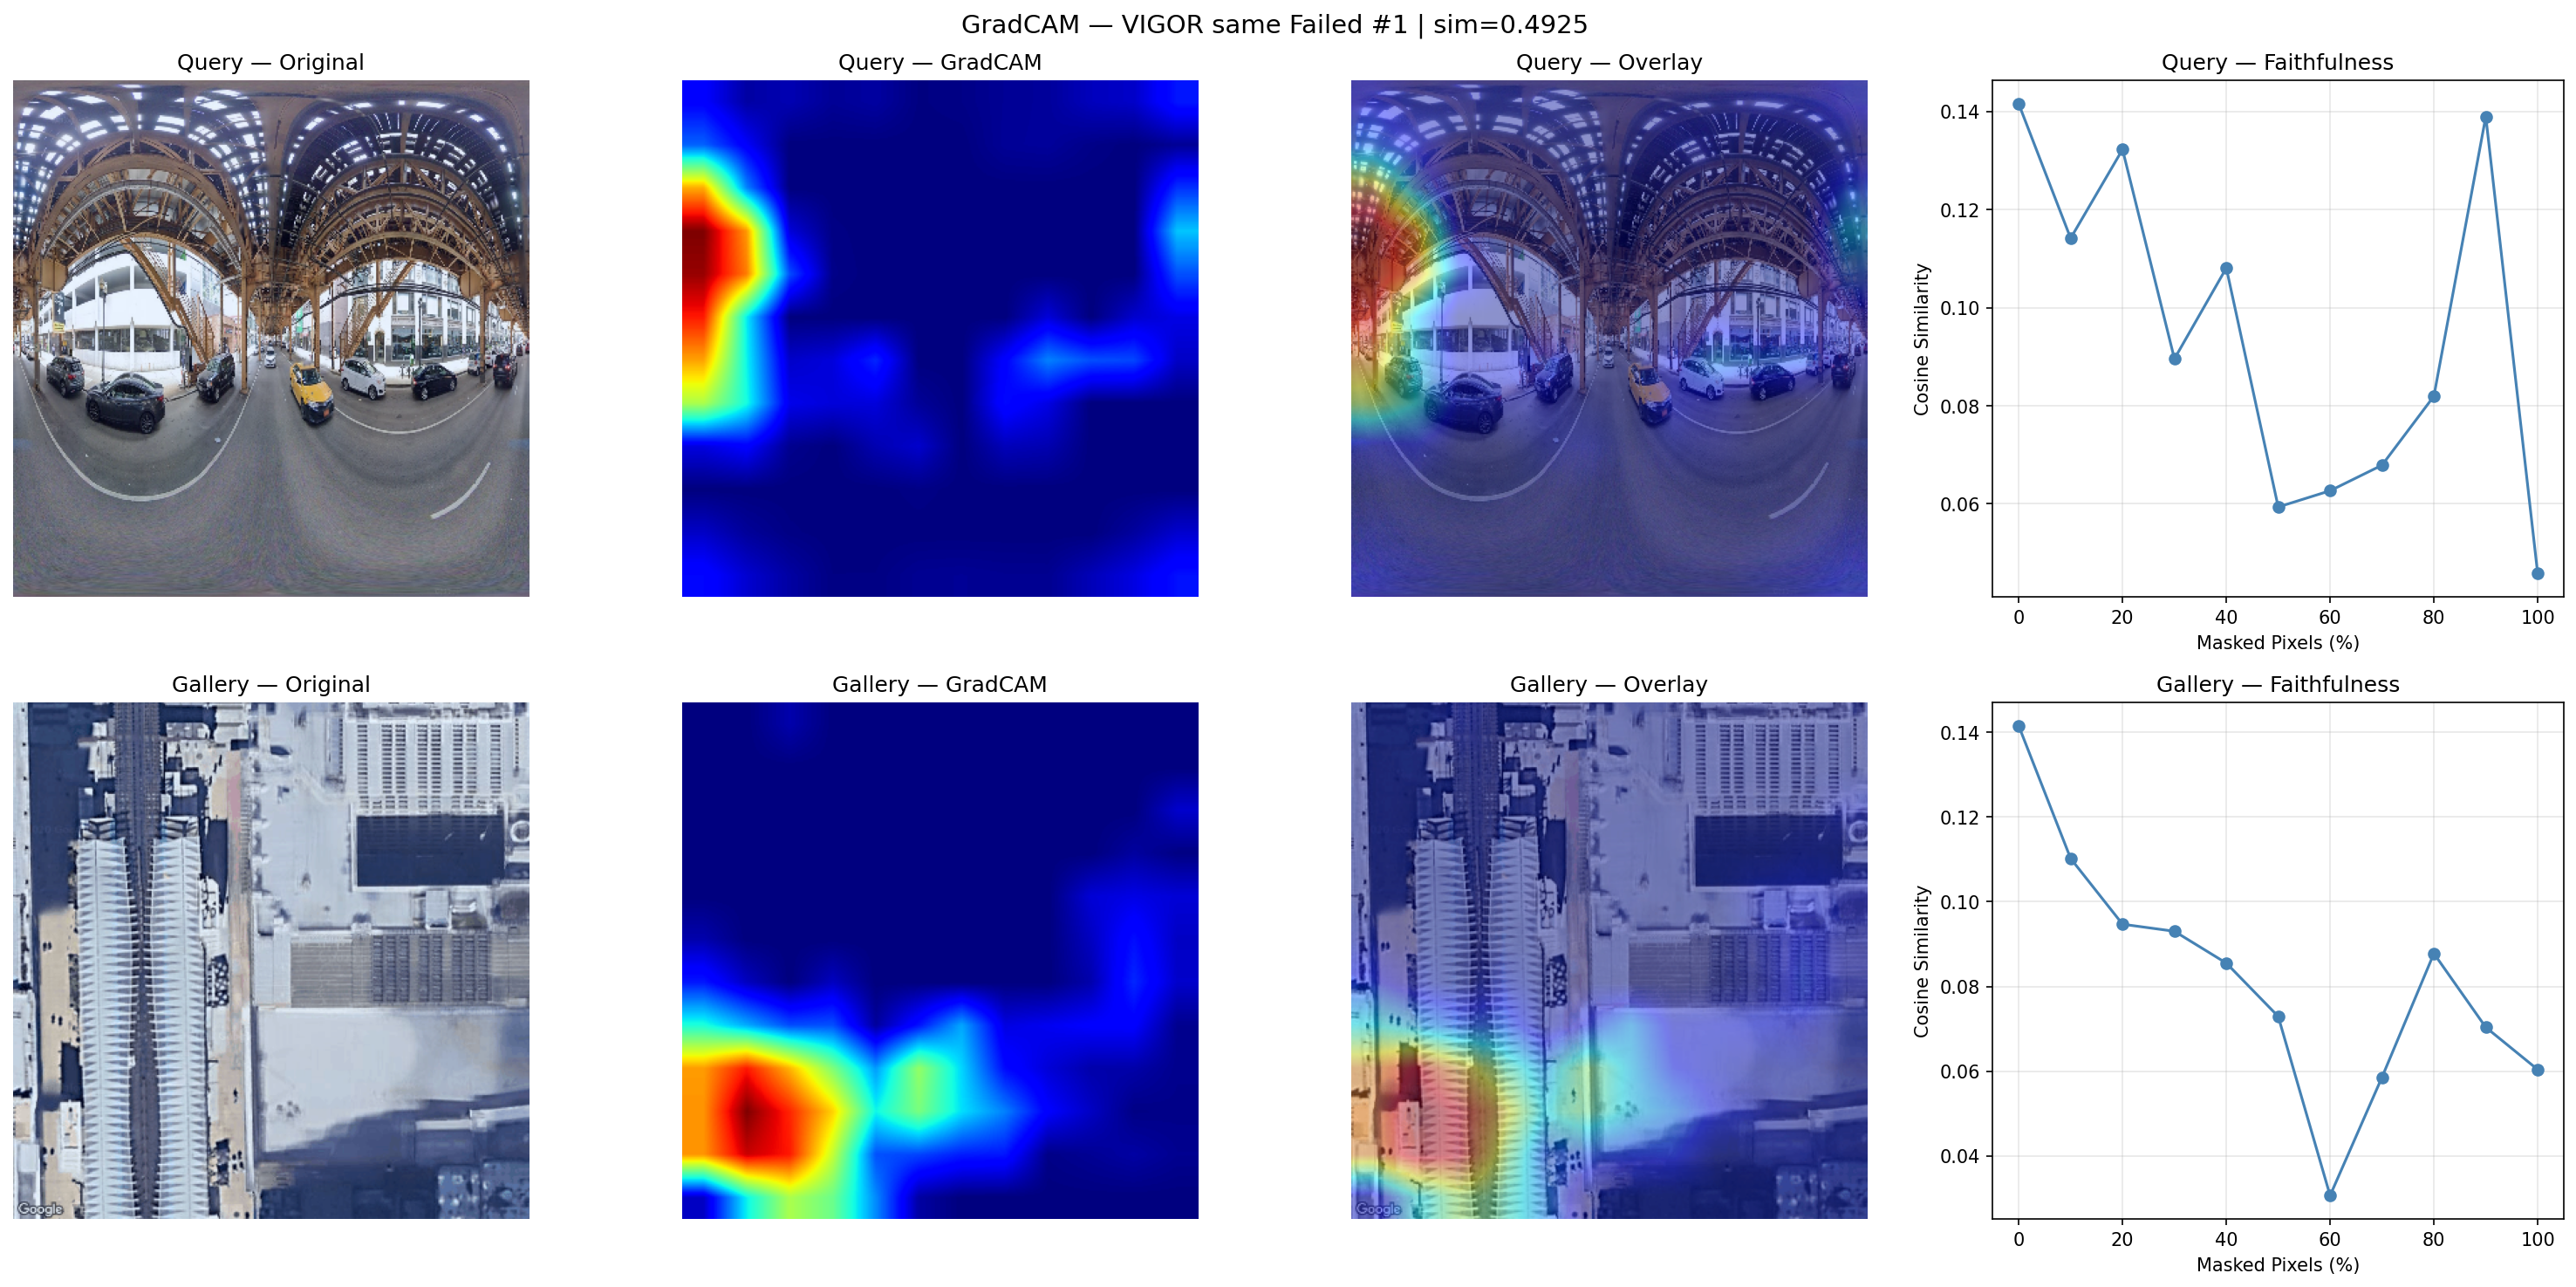
\includegraphics[width=\linewidth]{figures/gradcam/vigor_same_failed_01.png}
    \caption{Failed (sim=0.49)}
\end{subfigure}
\caption{Grad-CAM on VIGOR. (a) Successful: street boundary features map to satellite. (b) Failed: elevated rail structure (invisible from satellite) dominates attention; V-shaped faithfulness.}
\label{fig:gradcam_vigor}
\end{figure}

\subsection{Occlusion Sensitivity Analysis}

\paragraph{University-1652, Successful Matches (Figure~\ref{fig:occ_u1652}).}
Importance maps identify the same regions as Grad-CAM (building rooftop geometry), cross-validating both methods.
Heatmaps are coarser (blocky, 64px patch) but spatially consistent.
Faithfulness: clean monotonic decline (${\sim}0.89 \to {\sim}0.35$).

\paragraph{University-1652, Failed Matches (Figure~\ref{fig:occ_u1652}).}
The gallery map reveals fixation on a structurally insignificant background cluster.
Gallery faithfulness shows a paradoxical \emph{spike} at ${\sim}80\%$ masking: removing misleading pixels temporarily \emph{improves} similarity, confirming the model anchored on noise.

\paragraph{VIGOR, Successful Matches (Figure~\ref{fig:occ_vigor}).}
Concentrated importance on property boundaries and intersections.
Sharp initial faithfulness drop within the first 20\% of masking confirms that a small set of key pixels drives correct retrieval.

\paragraph{VIGOR, Failed Matches (Figure~\ref{fig:occ_vigor}).}
Erratic faithfulness: similarity \emph{climbs} to a peak at 90\% masking, proving complete feature confusion.

\begin{figure}[t]
\centering
\begin{subfigure}[t]{0.49\linewidth}
    
\includegraphics[width=\linewidth]{figures/occlusion/u1652_successful_01.png}
    \caption{Successful (ID=0003, sim=0.89)}
\end{subfigure}
\hfill
\begin{subfigure}[t]{0.49\linewidth}
    
\includegraphics[width=\linewidth]{figures/occlusion/u1652_failed_01.png}
    \caption{Failed (true=0010, ret.=-001)}
\end{subfigure}
\caption{Occlusion Sensitivity on University-1652. (a) Successful: building geometry identified, monotonic faithfulness. (b) Failed: gallery faithfulness spikes at 80\%, confirming misleading features.}
\label{fig:occ_u1652}
\end{figure}

\begin{figure}[t]
\centering
\begin{subfigure}[t]{0.49\linewidth}
    
\includegraphics[width=\linewidth]{figures/occlusion/vigor_same_successful_01.png}
    \caption{Successful (sim=0.57)}
\end{subfigure}
\hfill
\begin{subfigure}[t]{0.49\linewidth}
    
\includegraphics[width=\linewidth]{figures/occlusion/vigor_same_failed_01.png}
    \caption{Failed (sim=0.49)}
\end{subfigure}
\caption{Occlusion Sensitivity on VIGOR. (a) Successful: sharp faithfulness drop validates boundary attention. (b) Failed: erratic curve with paradoxical similarity increase at 90\% masking.}
\label{fig:occ_vigor}
\end{figure}

%──────────────────────────────────────────────────────────────────────────────
\section{Discussion and Conclusions}
\label{sec:discussion}

\subsection{Cross-Validation of XAI Methods}

A central finding is that Grad-CAM and Occlusion Sensitivity consistently highlight the same spatial regions despite fundamentally different principles (gradient backpropagation vs.\ input perturbation).
This convergence significantly strengthens confidence that the identified regions reflect genuine model behaviour rather than method-specific artifacts.
Table~\ref{tab:method_comparison} summarizes the complementary strengths and weaknesses of each method.

\begin{table}[h]
\caption{Comparison of the two XAI methods applied in this study.}
\label{tab:method_comparison}
\centering
\small
\begin{tabular}{lcc}
\toprule
\textbf{Property} & \textbf{Grad-CAM} & \textbf{Occlusion Sensitivity} \\
\midrule
Type & White-box (gradient) & Black-box (perturbation) \\
Compute cost & 1 fwd + 1 bwd pass & 121 positions $\times$ batched fwd \\
Heatmap quality & Smooth, continuous & Coarse, blocky (64px patch) \\
Spatial resolution & $12\times12$ (from Stage 4) & $11\times11$ (stride 32) \\
Causal evidence & Indirect (correlational) & Direct (interventional) \\
Faithfulness curves & Post-hoc (external) & Native (built-in) \\
Architecture req. & Needs conv layers & Model-agnostic \\
\bottomrule
\end{tabular}
\end{table}

\subsection{Failure Mode Taxonomy}

Our analysis identifies two distinct and interpretable failure modes:

\paragraph{Mode 1: Diffuse Gallery Attention (University-1652).}
When the model retrieves the wrong satellite image, the gallery Grad-CAM activation spreads uniformly across the image.
The model cannot localize a discriminative region because the incorrect gallery image genuinely lacks a structure matching the query's attended features.
This manifests quantitatively as flat faithfulness curves and low-amplitude importance maps.
Interestingly, the \emph{query} heatmap remains focused even in failed cases. The failure originates not from the query encoder but from the absence of a matching anchor in the wrong gallery image.

\paragraph{Mode 2: Cross-View Invisible Features (VIGOR).}
In VIGOR failures, the model attends to structures prominent from street level (e.g., elevated rail infrastructure, overhead signage) but invisible from the satellite perspective.
This creates a fundamental cross-view mismatch: the query embedding encodes features with no spatial counterpart in any satellite image.
Non-monotonic faithfulness curves, where masking certain regions \emph{improves} similarity, provide quantitative proof that these features actively mislead the retrieval by inflating similarity to an incorrect gallery image.
This failure mode is structurally different from Mode~1: here the problem lies in the query encoder attending to view-dependent features, not in the gallery lacking information.

\subsection{Dataset Difficulty and XAI Patterns}

University-1652 (drone $\leftrightarrow$ satellite) presents a moderate viewpoint gap where both views are roughly top-down.
Attended features (rooftop geometry, building footprints) transfer well across views, producing smooth and monotonic faithfulness curves for successful matches.
The model achieves R@1 $>$ 92\% by reliably mapping 3D building structure to 2D satellite footprints.

VIGOR (street $\leftrightarrow$ satellite) presents an extreme ${\sim}90^\circ$ viewpoint gap.
Even successful matches show noisier faithfulness curves, reflecting the inherent difficulty of cross-view correspondence.
The model succeeds when it identifies ground-level structural boundaries (fences, road edges, property lines) that are visible from both perspectives.
The significantly lower R@1 (77.86\% same-area, 61.71\% cross-area) quantitatively confirms that the street-to-satellite task is fundamentally harder than drone-to-satellite.

\subsection{Computational Challenges}

Evaluating the VIGOR dataset required computing a similarity matrix of size $52{,}605 \times 90{,}618$ (same-area), requiring ${\sim}19$~GB of contiguous memory.
This exceeded GPU capacity, necessitating a streaming chunked approach with explicit memory management.
Additionally, feature extraction for VIGOR took ${\sim}2$~hours on an A100 due to Drive I/O latency when reading ${\sim}90{,}000$ small image files.
We mitigated this with aggressive DataLoader pipelining (16 workers, prefetch factor 4, persistent workers) and caching all features/metrics to Drive for session persistence.

\subsection{Limitations and Future Work}

\paragraph{Limitations.}
(1) All 5 successful U1652 pairs share the same building class (ID~0003) due to greedy sequential selection. This demonstrates viewpoint robustness but limits visual diversity in the report.
(2) Occlusion resolution ($64{\times}64$ patch, stride~32) is deliberately coarse for computational efficiency, producing visibly blocky maps; finer resolution would require ${\sim}300$ forward passes per image.
(3) We analyze a single architecture (ConvNeXt-Base); findings may not generalize to vision transformers or hybrid architectures.
(4) Faithfulness curves use pixel-level masking applied to the GradCAM/Occlusion importance maps, which conflates spatial importance with the masking strategy.

\paragraph{Future Directions.}
To address the identified failure modes:
(i) Multi-scale feature pyramids with hierarchical attention could prevent the network from over-indexing on background distractors in aerial views.
(ii) Incorporating explicit depth estimation or 3D point-cloud priors could bridge the geometric disconnect in street-to-satellite matching, ensuring the model does not encode features from overhead structures that have no satellite counterpart.
(iii) View-consistency regularization losses that penalize high similarity between features present in only one viewpoint could improve cross-view robustness.
(iv) Applying additional XAI methods (LIME, Integrated Gradients) could provide further validation of the identified spatial patterns.

\subsection{Conclusion}

We presented a systematic XAI analysis of cross-view geo-localization using Grad-CAM and Occlusion Sensitivity across two datasets and eight operational scenarios.
Both methods consistently identify building geometry and structural boundaries as the discriminative features driving successful matching.
Failure modes are interpretable and distinct: diffuse gallery attention for incorrect matches (the wrong image lacks discriminative structure) and cross-view invisible feature fixation for extreme perspective gaps (the model attends to structures absent from satellite view).
Faithfulness curves provide quantitative evidence that validates the heatmaps and, crucially, reveals cases where attended features actively \emph{mislead} rather than support the retrieval decision.
These findings provide actionable insights for improving cross-view geo-localization architectures and demonstrate the value of applying multiple complementary XAI methods to complex retrieval systems.

%──────────────────────────────────────────────────────────────────────────────

\bibliography{references}
\bibliographystyle{iclr2025_conference}

\end{document}
